\documentclass[]{article}
\usepackage{graphicx}
\usepackage{amsmath,amsfonts,amssymb}
\usepackage[many]{tcolorbox}
\usepackage[%
margin=2cm,
includefoot,
bottom=2.55cm,
top=2.025cm,
headsep=0.5cm,
footskip=0.65cm
]{geometry}

\definecolor{myblue}{RGB}{0,46,142}

\newtcolorbox[auto counter]{mytheorem}[1][]{%
	enhanced jigsaw,
	colback=white,
	colframe=myblue,
	coltitle=myblue,
	fonttitle=\bfseries,
	sharp corners,
	detach title,
	enlarge left by=18mm,
	width=\linewidth-18mm,
	underlay unbroken and first={%
		\node[above,text=myblue,font=\bfseries,align=center] at ([xshift=-.5\textwidth,yshift=-7mm]interior.north) {\thetcbcounter};
	},
	breakable,
	pad at break=1mm,
	#1,
	code={\ifdefempty{\tcbtitletext}{}{\tcbset{before upper={\tcbtitle\par\medskip}}}},
}
\graphicspath{ {./images/} }


%opening
\title{L-16: Orthogonal Vectors and Subspaces}
\author{Aahan Singh Charak\\Computer Science Grad}

\begin{document}
\maketitle
\section{Least Squares}
\vspace{10pt}
\subsection{Some more things about projection matrices.}
\vspace{10pt}

\begin{itemize}
	\item If b is in column space of A, P.b=b
	\item If $b\perp b$, P.b=0
\end{itemize}

\vspace{10pt}

\subsubsection{P.b=b}
\vspace{10pt}

$N(A^T)\perp C(A)$\\

\noindent
$P.b=A{(A^TA)}^{-1}A^Tb$\\

\noindent
$\therefore P.b=0$

\vspace{10pt}

\subsubsection{P.b=b}
\vspace{10pt}

$P.b=A{(A^TA)}^{-1}A^TAx$ \{b=Ax\}\\

\noindent
$P.b=A.x$\\

\noindent
$\therefore P.b=b$\\
	
	
\subsection{I-P projection matrix}

P is the projection matrix which projects a vector b onto the column space of matrix A. The other projection component lies on null space of A transpose, since $n(A^T)$ is orthogonal to the column space of A.
\vspace{10pt}
\subsubsection{Proof that I-P is projecting onto the null space of A transpose}
\vspace{10pt}
Suppose vector b lies on the column space of A.\\

\noindent
$\therefore P.b=b$\\

\noindent
(I-P).b = I.b - P.b\\
=b - b\\
=0\\

\noindent
(I-P).b = 0 means that there is no component of b vector along that subspace. Therefore, I-P must have projected onto $n(A^T)$, which is orthogonal to the column space of A.\\

\textbf{Prove the same using the logic that P.y=0, where y lies on $n(A^T)$}

\vspace{10pt}

\section{Geometric Least Squares}
\vspace{10pt}
\begin{center}
	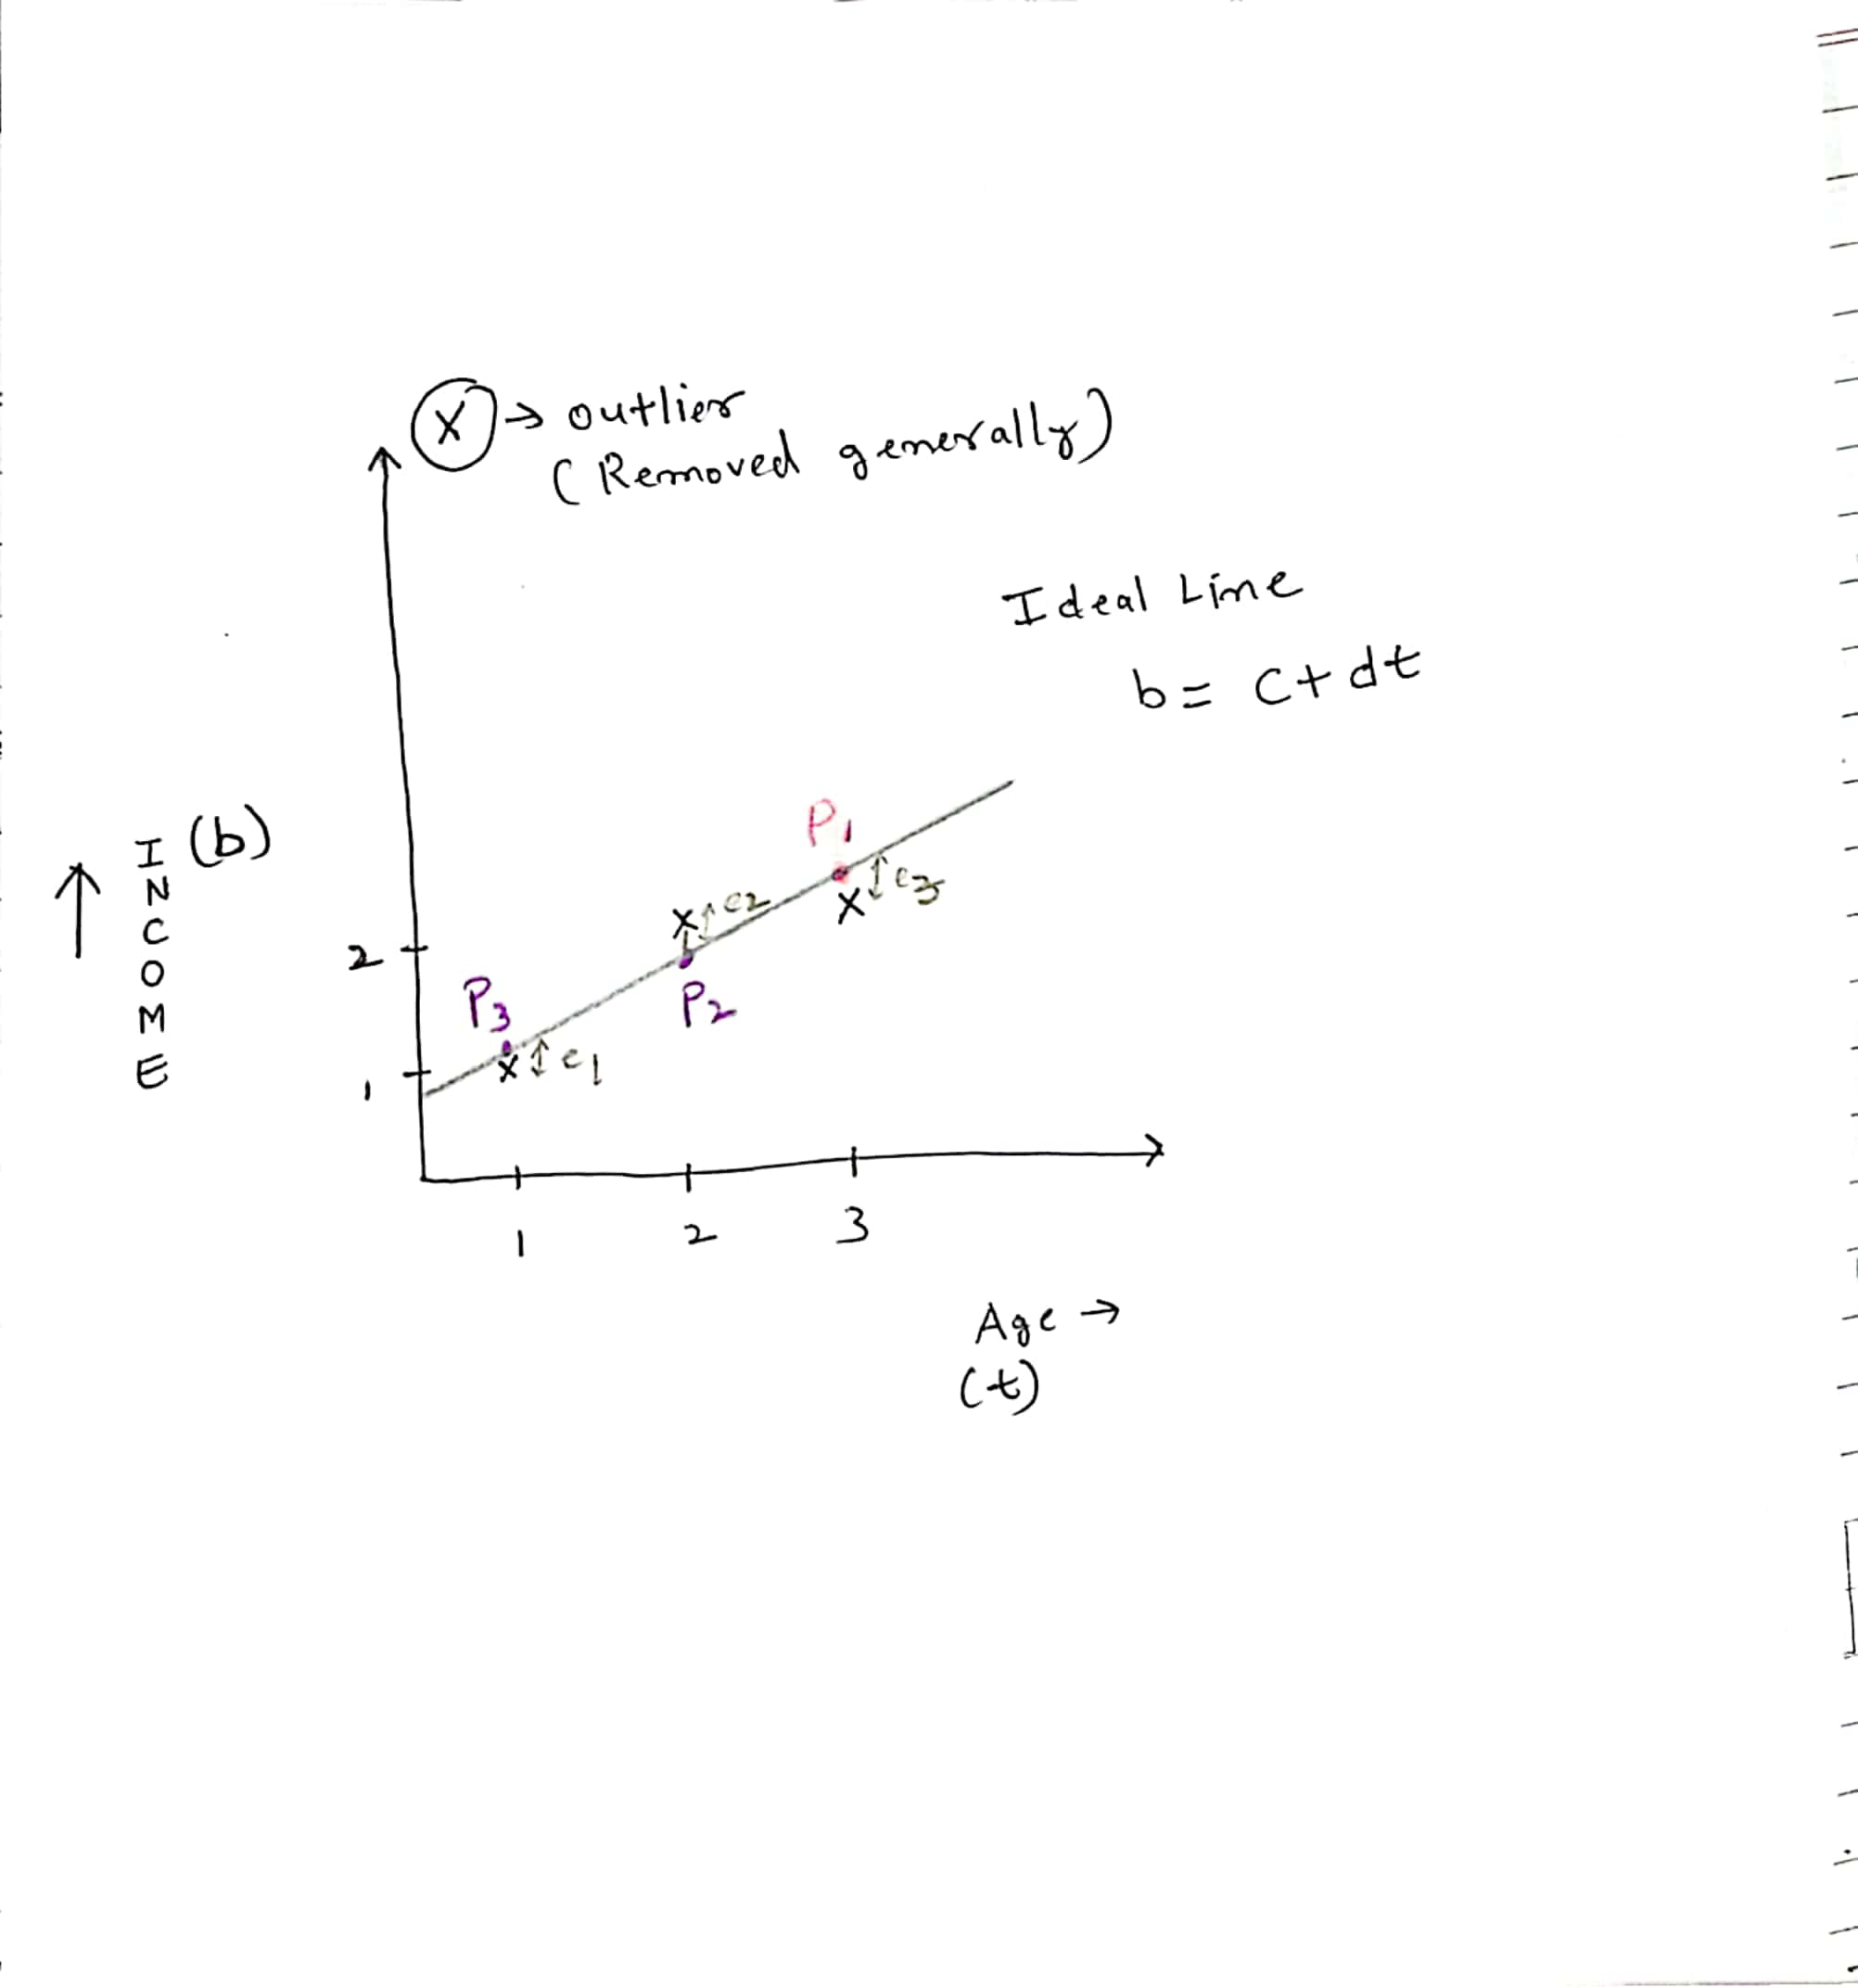
\includegraphics[scale=.18]{least_squares}
\end{center}
\vspace{10pt}

\noindent
In the figure above, we can see three points at co-ordinates (1,1), (2,2), (3,2). The task here is to find a line which best fits these points,so that the error is minimum.\\

\noindent
b=c+dt is the required line in this case. The ideal line equation for the three given points would be:\\

\noindent
C+D=1\\
C+2D=2\\
C+3D=2\\

\noindent
It is visibly obvious that there is no solution to these set of equations, even if we proceed by normal gaussian elimination.\\

\noindent
We can rewrite the matrix in Ax=b form as:\\

\noindent
\[
\begin{bmatrix}
	1 & 1\\
	1& 2\\

	1&3
	
\end{bmatrix}\begin{bmatrix}
C\\
D
\end{bmatrix}=\begin{bmatrix}
1\\
2\\
3
\end{bmatrix}
\]\\

\noindent
Now, b does not lie in column space of the A matrix. So we need to find $\hat{x}$, which is an estimated solution to the nearest projection of b onto the column space of A(best line).\\

\[
\hat{x}= \begin{bmatrix}
	\hat{C}\\
	\hat{D}
\end{bmatrix},
where \ the \ hat \ sign \ on \ C \ and \ D  \ means \ that \ they \ are \ estimated \ values \ for \ the \ best \ line.
\]\\

\noindent
From lecture 15 we already know that:\\

\noindent
$A^TA\hat{x}=A^Tb$\\

\noindent
Substituting values we get:\\

\noindent
\[
A^TA=\begin{bmatrix}
	3&6\\
	6&14
\end{bmatrix}
\]\\

\[
A^Tb=\begin{bmatrix}
	5\\
	11
\end{bmatrix}
\]\\

\noindent
We get two equations from these:\\

\noindent
$3\hat{C}+6\hat{D}=5$\\
$6\hat{C}+14\hat{D}=11$\\

\noindent
Solving these two equations, we get:\\

\noindent
$\hat{C}=\frac{2}{3}$\\

\noindent
$\hat{D}=\frac{1}{2}$\\

\noindent
The resulting equation is :
p=$\frac{2}{3}+\frac{1}{2}t$\\

\noindent
The points on the line p = $[\frac{7}{6}, \frac{5}{3}, \frac{13}{6}]$\\

\noindent
The error vector e = $[\frac{-1}{6}, \frac{2}{6}, \frac{-1}{6}]$\\

\noindent
We can verify that b=p+e. This means that $e \perp C(A)$\\

\vspace{10pt}

\section{Least Squares Calculus Approach}
\vspace{10pt}

\noindent
Under the calculus approach, we have to minimize the sum of squared error vector function. We square in order to not cancel out the -ve and +ve values (we can take absolute too).\\

\noindent
The objective function is given as:\\

\noindent
$min({||Ax-b||)}^2=min({||e||}^2)$\\

\noindent
$=min({e_1}^2+{e_2}^2+{e_3}^2)$

\noindent
$=min({(C+D-1)}^2+{(C+2D-2)}^2+{(C+3D-2)}^2)$\\

\noindent
Taking partial derivative w.r.t C, we get:\\

\noindent
\begin{equation}
	\frac{\partial F}{\partial C} = 6C+12D-10
\end{equation}

\noindent
Setting partial derivative to zero gives:\\

\noindent
3C+6D=5\\

\noindent
\begin{equation}
	\frac{\partial F}{\partial D} = 12C+28D-22
\end{equation}

\noindent
12C+28D=22\\

\noindent
We can solve these equations the same way as in the algebraic approach.

\vspace{10pt}
\section{Bonus Proofs}
\vspace{10pt}
\subsection{If A has independent columns, then $A^TA$ is invertible}
\vspace{10pt}
Suppose $A^TAx=0$ for some x.\\

\noindent
Multiply both sides by $x^T$\\

\noindent
$x^TA^TAx=0$\\
${(Ax)}^TAx=0$\\
$||Ax||^2=0$\\
$A.x=0$ [$\because$ length square is zero. length is zero, which means vector is zero, as length is component squared.]\\

\noindent
A has independent columns(given) and A.x=0. This must mean x is zero.

\noindent
$A^TAx=0$ $\implies$ x=0

\noindent
This means $A^TA$ is invertible if A has independent columns.

\noindent
\textbf{Q.E.D}





\end{document}